\chapter{Intersection Algorithms\label{intersect}}

In this chapter we are going to see a collection of algorithms to compute the intersection of two \textbf{sorted} lists, taken from the chapter six of "Pearl of Algorithm Engineering" by Paolo Ferragina, published by Cambridge University Press \citep{Ferragina_2023}. \\
We will first look at two of the most commonly used search algorithms, since we cannot intersect without searching. \\

\section{Search Algorithms}

\subsection{Binary Search \label{sec:binsearch}}

\begin{figure}[ht] 
    \begin{center}
        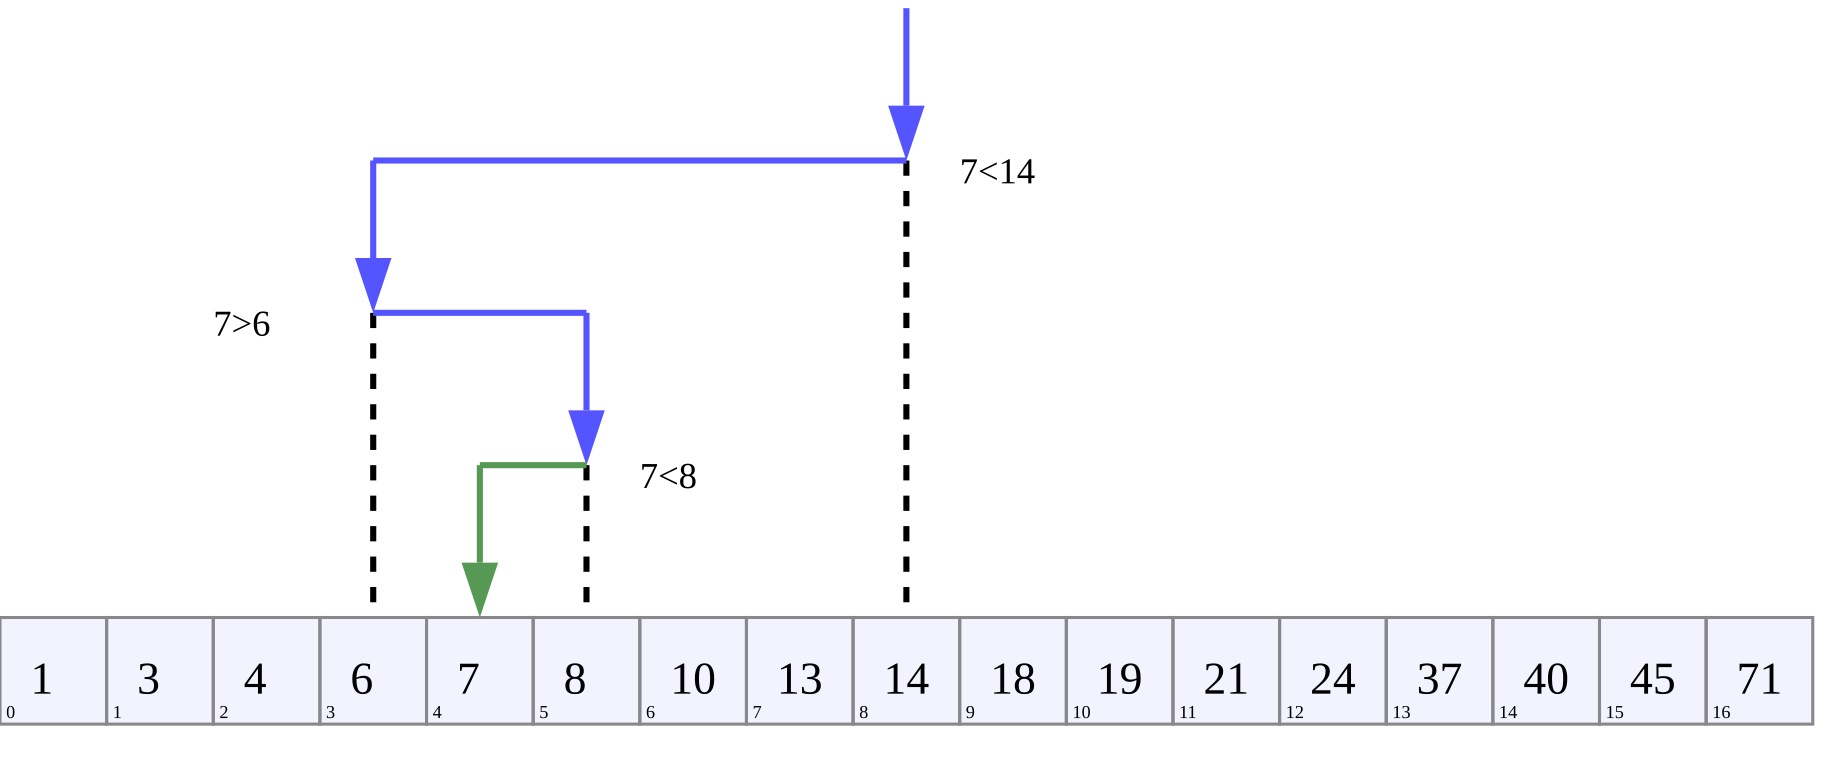
\includegraphics[width=.8\textwidth]{imgs/Binary_Search_Depiction.png}
        \caption{Binary search algorithm, source: \href{https://en.wikipedia.org/wiki/Binary_search}{Wikipedia}\label{fig:binsearch}}
    \end{center}
\end{figure}

Binary search, also known as logarithmic search or binary chop, is a search algorithm that finds the position of a target value within a sorted array: it compares the target to the middle element of the array and, if they are not equal, it eliminates half of the search space by discarding either the left or right half, depending on whether the target value is less than or greater than the middle element. This process is repeated by iteratively searching into the remaining sub-array until the target value is found or the search space is empty. The pseudocode for the algorithm can be seen at \textit{Algorothm 1} \brref{alg:binsearch}.\\
Binary search runs in logarithmic time in the worst case, doing $O(\log n)$ comparisons, where $n$ is the number of elements in the array, making it much faster than linear search with large arrays thanks to its scaling.\\

\begin{algorithm}
    \captionsetup{labelsep=newline}
    \caption{Pseudocode for binary search algorithm \label{alg:binsearch}}
    \begin{algorithmic}[1]
        \State looking for element $key$
        \State let $L=0$ \Comment{First half}
        \State let $R=n-1$ \Comment{Second half}
        \While{$L\leq R$}
            \State $m=\lfloor (L+R)/2 \rfloor$
            \If{$A[M] < key$}
                \State let $L=m+1$
            \ElsIf{$A[M] > key$}
                \State $R = m - 1$
            \Else
                \State \Return $m$ \Comment{Found}
            \EndIf
        \EndWhile
        \State \Return false \Comment{Not found}
    \end{algorithmic}
\end{algorithm}

\subsection{Exponential Search}

\begin{figure}[H] 
    \begin{center}
        \includegraphics[width=.8\textwidth]{imgs/exponential_search.png}
        \caption{exponential search algorithm, source: \href{https://www.tutorialspoint.com/data_structures_algorithms/exponential_search.htm}{Tutorialspoint}\label{fig:expsearch}}
    \end{center}
\end{figure}

Exponential search, also called doubling or galloping search, is an algorithm for searching sorted, unbounded lists: there are numerous implementations, most common being determining a sub-array into which the \verb|key| may resides in and performing a binary search \brref{sec:binsearch} within its range.\\
To be more precise: we go trough the list in exponentially increasing steps, with a factor of $2^k$ such that we first look into \verb+list[0]+, then \verb+list[1]+, then \verb+list[2]+, \verb+list[4]+, \verb+list[8]+, following with \textit{16}, \textit{32}, \textit{64}, \textit{128} and so on until we find a value that is greater than the \verb|key|. Once we find it, we perform a binary search between the previous jump and the current (or the end of the array): $2^{k-1} \leq key \leq min(2^{k},n)$.

The algorithm can be more efficient than binary search, as it runs in $O(\log i)$ time, where $i$ is the index of the element being searched for, which could be half if not less than $n$.\\
The pseudocode can be seen at \textit{Algorithm 2} \brref{alg:expsearch}.\\

\begin{algorithm}
    \captionsetup{labelsep=newline}
    \caption{Pseudocode for exponential search algorithm \label{alg:expsearch}}
    \begin{algorithmic}[1]
        \State looking for element $key$
        \State let $i=0$ 
        \State let $k=0$
        \While{($key>list[i+2^k]$ and $i<n$)} 
            \State $i=i+2^k$ \Comment Gallop to next step
            \State $k=k+1$ \Comment Increment exponent
        \EndWhile
        \If{$i<n$}
            \State binary\_search($list$, $key$, $i$, $min(i+2^k,n)$) 
        \Else
            \State \Return false \Comment{Not found}
        \EndIf
    \end{algorithmic}
\end{algorithm}

